\documentclass[conference]{IEEEtran}
\IEEEoverridecommandlockouts
% The preceding line is only needed to identify funding in the first footnote. If that is unneeded, please comment it out.
\usepackage{cite}
\usepackage{amsmath,amssymb,amsfonts}
\usepackage[super]{nth}
\usepackage{algorithmic}
\usepackage{graphicx}
\usepackage{textcomp}
\usepackage{xcolor}
\def\BibTeX{{\rm B\kern-.05em{\sc i\kern-.025em b}\kern-.08em
    T\kern-.1667em\lower.7ex\hbox{E}\kern-.125emX}}
\begin{document}

\title{\LARGE \bf VirNet: Sequence model for viral identification}

\author{
	\IEEEauthorblockN{Aly O. Abdelkareem}
	\IEEEauthorblockA{\textit{Department of Computer Engineering} \\
		\textit{Ain Shams University}\\
		Cairo, Egypt \\
		aly.osama@eng.asu.edu.eg}
	\and
	\IEEEauthorblockN{Mostafa Elaraby}
	\IEEEauthorblockA{\textit{Microsoft Research}\\
		Cairo, Egypt \\
		a-moelar@microsoft.com}
	\and
	\IEEEauthorblockN{Mahmoud I. Khalil}
	\IEEEauthorblockA{\textit{Department of Computer Engineering} \\
		\textit{Ain Shams University}\\
		Cairo, Egypt \\
		mahmoud.khalil@eng.asu.edu.eg}
	\and
	\IEEEauthorblockN{Hazem M. Abbas}
	\IEEEauthorblockA{\textit{Department of Computer Engineering} \\
		\textit{Ain Shams University}\\
		Cairo, Egypt \\
		hazem.abbas@eng.asu.edu.eg}
	\and
	\IEEEauthorblockN{Ali H. A. Elbehery}
	\IEEEauthorblockA{\textit{Institute of Virology} \\
		\textit{HelmholtzZentrum München}\\
		München, Germany \\
		aelbehery@aucegypt.edu}
}

%\author{%
%	Aly O. Abdelkareem$^{1}$, Mahmoud I. Khalil$^{2}$, Mostafa Elaraby$^{3}$, Hazem M. Abbas$^{4}$ and Ali H. A. Elbehery$^{5}$% <-this % stops a space
%	\thanks{$^{1}$Aly O. Abdelkareem is with department of computer engineering in Faculty of Engineering, Ain Shams University
%		{\tt\small aly.osama@eng.asu.edu.eg}}%
%	\thanks{$^{2}$Mahmoud I. Khalil is with department of computer engineering in Faculty of Engineering, Ain Shams University}%
%	\thanks{$^{3}$Mostafa Elaraby is a Research Software Development Engineer in Microsoft Advanced Research Lab in Cairo}%
%	\thanks{$^{4}$Hazem M. Abbas is with department of computer engineering in Faculty of Engineering, Ain Shams University}%
%	\thanks{$^{5}$Ali H. A. Elbehery is in Institute of Virology, Helmholtz Zentrum München{\tt\small aelbehery@aucegypt.edu} }
%}

\maketitle             

\begin{abstract}\\Metagenomics shows a promising understanding of function and diversity of the microbial communities due to the difficulty of studying microorganism with pure culture isolation. Moreover, the viral identification is considered one of the essential steps in studying microbial communities. Several studies show different methods to identify viruses in mixed metagenomic data and phages in host genomes, using homology and statistical techniques. These techniques have many limitations due to viral genome diversity. In this work, we propose a sequence deep neural model for viral identification of metagenomic data. For testing purpose, we generated fragments of viruses and bacteria from RefSeq genomes with different lengths to find the best hyperparameters of our model. Then, we simulated both microbiome and virome high throughput data from our test-set genomes in order to validate our method. %Finally, we applied our tool to a case study of two types of metagenomic data such as Roche 454 and Illumina.
We compared our tool to the state-of-the-art statistical tool for viral identification and found it performed much better regarding accuracy and speed on the same testing data. This tool will help us in growing our insights into natural viruses of microbial communities.
\end{abstract}
\begin{IEEEkeywords}
metagenomics; deep learning; virus; sequence model; classification 
\end{IEEEkeywords}


\section{Introduction}

Metagenomics is the cultivation-independent analysis of the genetic information of the collective genomes of the microbes within a given environment based on its sampling \cite{izard2014metagenomics}. There is a little portion of microbial organisms identified due to the difficulty in studying them using pure culture isolation. This methodology has been constrained to less than 1\% of host cells and is biased to certain species \cite{labonte2015single}.
% https://www.the-scientist.com/daily-news/most-gut-microbes-can-be-cultured-33581
Metagenomic analysis process demonstrates a promising understanding of different microorganisms. It answers some questions about microorganisms in the collection such as Who is there?, What can they do? Besides, what can they potentially do?.

Microorganisms are found everywhere on earth, and they are critical in our life. They are essential to our life. In this study, our interest is in Prokaryotic Microorganisms (e.g. Bacteria and Archaea) and viruses. Bacteria are unicellular and microscopic organisms that reproduce by binary fission. On the other hand, viruses are typically submicroscopic consists of genetic materials either DNA or RNA surrounded by a protective coat of proteins and can only replicate inside living host cells as they lack metabolic enzymes and equipment for making proteins, such as ribosomes. The bacterial genomes contain about 200 to a few thousand genes, while the tiniest viral genomes have only three genes and the largest have hundred to 2000 genes. 

Viruses have an impact on different microbial communities, and virus-host interaction can change many ecosystems such as human health and aquatic life. Viruses that infect bacteria are called bacteriophages or phages. Furthermore, phages are abundant in different microbiome communities. The viral infection starts when virus binds to a host cell and its genome integrated with the host cell genome. The integrated viral DNA called a provirus. It is reasonable to find that isolated viruses are just package of genes want to transit from one host cell to another. Scientists are using isolation and culture-independent techniques to study viral diversity and viral-host interactions in microbial communities. Those techniques have many limitations because there is no universal marker gene for viruses. Some reported most of the sequenced viruses in NCBI RefSeq are from 5\% of known phyla of prokaryotic hosts \cite{roux2015viral}.

High throughput sequencing technology is used for metagenomic studies which can generate massive amounts of short read sequences of microorganisms. We can sequence prokaryotic and viral cells in microbial communities regardless of cultivability of the cells at the same time in these samples. Sequencing microbial samples found viral sequences along with prokaryotic hosts. A study found 4-17\% virus sequences in human gut prokaryotic metagenomes \cite{minot2011human}. Moreover, Cellular contamination is quite frequent even with a careful purification of viral particles, and this is one of the main reasons why we need a tool that can differentiate between bacterial and viral sequences.

The broadly adopted technique to know who is in metagenomic data is to assemble the high throughput reads to contigs then search against a known genomic database using sequence alignment method in order to infer the type of microorganisms and the existence of species in a metagenomic sample. This approach is minimal because it only finds viruses closely related to those we already know. It is estimated that only about 15\% of viruses in the human gut microbiome and 10\% in the ocean have similarity to the known viruses \cite{ren2017virfinder}. 

Machine learning approaches have been used to classify and cluster data based on extracted features. The deep neural network is one of machine learning methods that are considered as a state of the art category for general classification problems. Deep learning shows significant improvements in several artificial intelligence tasks for example image classification, speech recognition, and natural language processing. Moreover, It shows significant results with genomic data \cite{angermueller2016deep}. \\

In this paper, we introduce a deep sequence model, VirNet, to identify viral sequences from a mixture of viral and bacterial sequences and purify viral metagenomic data from bacterial contamination as well. That will guide us to find new viruses and study their genomes, and beside of that, it answers many mysteries related to our understanding of their functionality and diversity in the ecosystem.

\section{Related Work}

There has been extensive prior work on viral identification. Recent work has focused on identifying phages in bacterial genomes. Several methods have used similarity search with the known genomes in order to find viral contigs. There are three types of recent tools:
\begin{enumerate}
	\item Phages from prokaryotic genomes
	\item Viral sequences in mixed metagenomic datasets
	\item Phages and Viral sequences. 
\end{enumerate} 

There are many methods to find phages from prokaryotic genomes such as Phage\_Finder \cite{fouts2006phage_finder}, Prophinder \cite{lima2008prophinder}, PHAST\cite{zhou2011phast}, and PhiSpy \cite{akhter2012phispy}. These tools are using similarity search to known viruses databases using features such as genes. Some of them such as PhiSpy integrates other features such as protein length, AT and GC skew, transcription strand direction and unique virus k-mers. They have many limitations as they failed to detect viral sequences in metagenomic data as the databases are outdated, limited and don't represent viral diversity in the environment. Moreover, It is not optimized to process a large number of contigs \cite{roux2015virsorter} as they depend on alignment and homology processing limitations. 

The second type is able to detect viral sequences in mixed metagenomic datasets such as VIROME \cite{wommack2012virome} and MetaVir\cite{roux2011metavir}. They are using similarity search with the databases as same as the first type and Also, they are searching against proteins. Some people are using DIAMOND \cite{buchfink2014Diamond} or Centrifuge \cite{kim2016centrifuge} as they are fast and efficient for microbial classification. The limitation of this approach is related to limited databases as they only search for known genomes. 

The third type is able to detect phages and viral sequences such as VirSorter \cite{roux2015virsorter}. VirSorter is using similarity search to viral databases and integrates other features such as viral hallmark gene, enrichment of viral-like genes, enrichment of uncharacterized genes which make it more accurate but it has many limitations such as it require at least 3 genes within the contig as the smallest virus genome contains 3 genes so it has the same limitations as previous techniques because of using homology strategy. Moreover, it cannot work with short fragments or contigs and it is very slow in processing metagenomic datasets. 

Recently VirFinder \cite{ren2017virfinder} applied machine learning techniques. VirFinder is a statistical method based on the logistic regression model. It uses the K-mer feature which is considered as a discrimination feature for different sequence problems. It shows a great success with short sequences too and They found a great k-mer similarity score with viruses within other prokaryotic genomes. 

% need to write deep learning techniques in fragments classification

In this paper, we are using deep learning techniques which is much more suitable to sequence problems and also shows significant improvements to other machine learning models. In deep neural networks, the model will extract the most appropriate features during training which lead to better identification accuracy. 

\section{Materials and Methods}

\subsection{Building training and testing dataset}
We downloaded viruses, bacteria and archaea genomes from RefSeq database then we divided them randomly into a train and test genomes with 80\% of total base pairs in training. Table \ref{table:genome_stats} shows the number of genomes we used in training and testing. We used all available viral genomes until Nov. \nth{1}, 2017 and a sample from prokaryotic genomes due to the huge number of available prokaryotic genomes. Then, we converted the viral genomes into non-overlapping fragments of different lengths n = \{100, 500, 1000, 3000\}. Beside that, we generated randomly an approximate number of prokaryotic non-overlapping fragments of the same lengths (Table \ref{table:fragments_stats}). We balanced the data of both classes using random under-sampling technique to avoid the deep neural network bias to the majority class. Figure \ref{fig:data_pipline} shows more details for data pipeline.

\begin{figure}
	\centering
	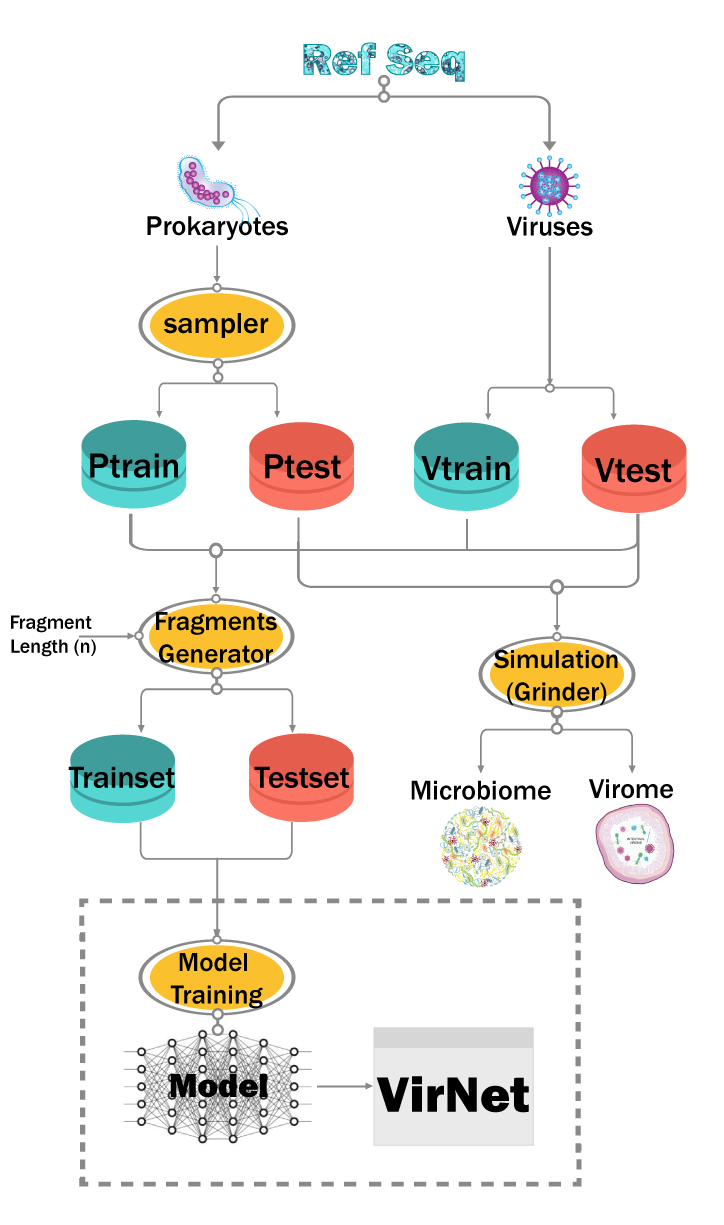
\includegraphics[width=\columnwidth]{imgs/data_pipeline.PNG}
	\caption{VirNet Data Pipeline}
	\label{fig:data_pipline}
\end{figure}

\begin{table}[h!]
	\centering
	\begin{tabular}{||c c c c||} 
		Genome & Train & Test & Total \\ [0.5ex] 
		\hline\hline
		Viruses & 7686  & 1870 & 9556 \\ 
		Prokaryotes & 143241  & 35543 & 178784  \\ [1ex] 
	\end{tabular}
	\caption{The number of used genomes from RefSeq}
	\label{table:genome_stats}
\end{table}

\begin{table}[h!]
	\centering
	\begin{tabular}{||c c c||} 
		Fragment Length (N) & Train & Test \\ [0.5ex] 
		\hline\hline
		100 bp & 2088863  & 527020  \\ 
		500 bp & 420857  & 106168  \\
		1000 bp & 212253  & 53528  \\
		3000 bp & 73163  & 18425  \\ [1ex] 
	\end{tabular}
	\caption{The number of fragments generated from viruses genomes}
	\label{table:fragments_stats}
\end{table}

\subsection{Generate simulated virome and microbiome}
Grinder \cite{angly2012grinder} is an open-source tool commonly used for generating a simulate amplicon and shotgun metagenomic datasets from reference genomes. 
We generated two metagenomic data of virome and microbiome of 1M reads and fragment length 100bp using Grinder with our reference test genomes to simulate shotgun metagenomic sequences in order to verify the ability of our tool to work on metagenomic data instead of fragments from the genomes. Moreover, we used Illumina error model indicated by mutation\_dist poly4 3e-3 3.3e-8 and mutation ratio 91:9 (9 indels for each 91 substitution mutations) because for Illumina indel errors occur more often than substitution errors \cite{laehnemann2015denoising}. Table \ref{table:simulate_stats} shows simulated data statistics.  \\

\begin{table}[h!]
	\centering
	\begin{tabular}{||c c c||} 
		& Microbiome & Virome \\ [0.5ex] 
		\hline\hline
		Bacteria Length & 75450367  bp  & 17551396 bp  \\
		Bacteria Genomes & 1488 & 422\\
		Bacterial reads & 803742 & 176059\\
		Viruses Length & 25133078 bp  & 52609236 bp  \\ 
		Viruses Genomes & 845 & 1870\\
		Viral reads & 196258 & 823941 \\  
		Viral Ratio & 25.00\% & 75.00\% \\ 
		Library coverage &  0.994x &  1.001x  \\
		Diversity (richness) & 2302 & 2726 \\ [1ex]
	\end{tabular}
	\caption{Grinder Simulated Metagenome}
	\label{table:simulate_stats}
\end{table}


%\subsection{Case Study: Real metagenomic data}
%We applied our tool to two real metagenomes as a case study
%\begin{enumerate}
%	\item \textbf{454}: Subtropical freshwater microbial and viral metagenome (SRR648314).\
%	\item \textbf{Illumina}: Lake Michigan virome (SRX995836).
%\end{enumerate}
%Our tool is able to read not only fasta files and fastq files. Furthermore, it is able to deal with paired-end reads i.e. if one of the two pairs is identified as a virus, the other should be the same. If there are conflicts between the classifications of the two pairs; this pair could be denoted as ambiguous.

\subsection{Deep Learning Model}
Recurrent neural networks (RNN), long short-term memory (LSTM) \cite{hochreiter1997long} and gated recurrent neural networks (GRU) \cite{chung2014empirical} can model complex sequences and have been used for sequence modeling problems. All these variations were used during to get the performing model over the input fragments. 

The deep learning model is implemented as an attentional encoder network (Figure \ref{fig:encoder}). An input sequence  $\mathbf{x = (x_{1} , \ldots{} , x_{m} )}$  and calculates a forward sequence of hidden states  ($\mathbf{\overrightarrow{h_{1}}}$,\ldots{},$\mathbf{ \overrightarrow{h_{m}}}$). The hidden states $\mathbf{\overrightarrow{h_{j}}}$  are averaged to obtain the attention vector $\mathbf{h_{j}}$ representing the context vector from the input sequence.

Embedding Layer maps discrete input words to dense vectors for computational efficiency before feeding this sequence to LSTM/GRU Layers. The attentional network could learn how to extract suitable features from the raw data and can attend to previous DNA nucleotide within the same input sequence. 

LSTM encoder have 3 gates to protect and control the cell state, the input gate denoted $\mathbf{i}$ which defines how much of the newly computed state you want to let through, forget gate denoted $\mathbf{f}$ that decides what information is to be kept and what is to be thrown away ,  the output of the update gate denoted $\mathbf{U}$ that's used to update the cell state and the output of the LSTM cell $\mathbf{o}$ .$\mathbf{W}$ is the recurrent connection at the previous hidden layer and current hidden layer and $\mathbf{C}$ is the internal memory of the unit  as shown in the following equations \newline
$\mathbf{i_{t}=\sigma(x_{t}U^i + h_{t-1}W^i)}$ \newline
$\mathbf{f_{t}=\sigma(x_{t}U^f + h_{t-1}W^f)}$ \newline
$\mathbf{o_{t}=\sigma(x_{t}U^o + h_{t-1}W^o)}$. 

GRU encoder is same as LSTM except it has only 2 gates, Reset gate denoted $\mathbf{r}$ that determines how to combine the new input with the previously saved input state and the update gate denoted $\mathbf{z}$ that defines the amount of information to keep around, as defined  in the following equations \newline
$\mathbf{z_{t}=\sigma(x_{t}U^z + h_{t-1}W^z)}$ \newline
$\mathbf{r_{t}=\sigma(x_{t}U^r + h_{t-1}W^r)}$ \newline
$\mathbf{\overline{h_{t}} = tanh(x_{t}U^h + (r_{t} * h_{t-1})W^h )}$ \newline
$\mathbf{ h_{t} = (1-z_{t})h_{t-1} +z_{t}\overline{h_{t}}}$.

The few numbers of gates in GRU makes it faster to converge than the LSTM on moderate data size. After trying both on this data, LSTM was outperforming the GRU model which was expected depending on the input data size.

The attentional neural model was trained with the DNA nucleotide bases with 100bp fragments. The model will then try to predict in a binary format whether this fragment is viral or non-viral.

The top-performing model (Figure \ref{fig:model_diagram}) consists of an input embedding layer of size 128 mapping input DNA nucleotide tokens into an embedding space, that is fed to a GRU layer. The forward sequence $\mathbf{\overrightarrow{h_{j}}}$ is then averaged together to create an attentional vector representing token context within the same fragment. A dropout layer was added after the attentional layer to avoid overfitting over the input data.
s
The input sequence is divided into 5 grams sized tokens these tokens are then treated as a single word.This single token is mapped as a point in the embedding space created during training the neural model.

During training, all parameters are optimised jointly using Adam to maximise the conditional probability of tokens found together to predict if an input sequence is viral or not.

In this model, an early stopping mechanism was used as a form of regularisation to avoid overfitting over the data while making more epochs over the data. The early stopping mechanism was used with patience of 3 non -improving consecutive epochs; the neural model will stop training while saving the latest improving checkpoint over the validation set defined.

\subsection{Hyperparameters optimization}

Model parameters affect the performance of the deep learning model, and they control the behaviour of the training algorithm as well. We selected the grid search technique in order to find the most suitable parameters. The grid search is considered a traditional technique for hyperparameters optimisation and it brute force different combinations. We ran several experiments on 20\% of our training set for 500 bp. Then, we divided it into training, validation, and testing set with the following percentages 70\%, 10\%, and 20\%. These experiments were designed to find the best parameters for the number of recurrent layers, the embedding size for each layer and the input sub-words (ngram). Our results are reported (Table \ref{table:hyper_results}) shows us that the best parameters setup was for 2 layers, 128 embedding size, and 5 ngram. 

We ran other experiments with the same parameters to check the ability of our model with other configuration, so we changed different parameters separately such as embedding size to 256 neurons, the number of layers to 3 and the recurrent cell type to GRU instead of LSTM. We found a slightly less accuracy and roc-auc scores but the training time was much more than the best parameters configuration as expected due to increasing number of neural network parameters.

\begin{table}[h!]
	\centering
	\begin{tabular}{||c c c c c||} 
		\#Layers & Embedding (\#Neurons) & Ngram & ROC-AUC & Accuracy \\ [0.5ex] 
		\hline\hline
		1      & 32                      & 3     & 0.8     & 73.66    \\
		1      & 32                      & 5     & 0.83    & 76.42    \\
		1      & 32                      & 7     & 0.79    & 72.11    \\
		1      & 64                      & 3     & 0.83    & 76.1     \\
		1      & 64                      & 5     & 0.83    & 75.98    \\
		1      & 64                      & 7     & 0.77    & 69.96    \\
		1      & 128                     & 3     & 0.83    & 75.76    \\
		1      & 128                     & 5     & 0.85    & 77.41    \\
		1      & 128                     & 7     & 0.78    & 70.93    \\
		2      & 32                      & 3     & 0.8     & 73.25    \\
		2      & 32                      & 5     & 0.83    & 76.49    \\
		2      & 32                      & 7     & 0.79    & 72.82    \\
		2      & 64                      & 3     & 0.81    & 73.96    \\
		2      & 64                      & 5     & 0.84    & 76.46    \\
		2      & 64                      & 7     & 0.78    & 72.53    \\
		2      & 128                     & 3     & 0.83    & 76.15    \\
		\textbf{2} & \textbf{128}            & \textbf{5} & \textbf{0.85} & \textbf{77.9} \\
		2      & 128                     & 7     & 0.78    & 70.63    \\[1ex]
	\end{tabular}
	\caption{Hyperparamters optimization results}
	\label{table:hyper_results}
\end{table}


\begin{figure}
	\centering
	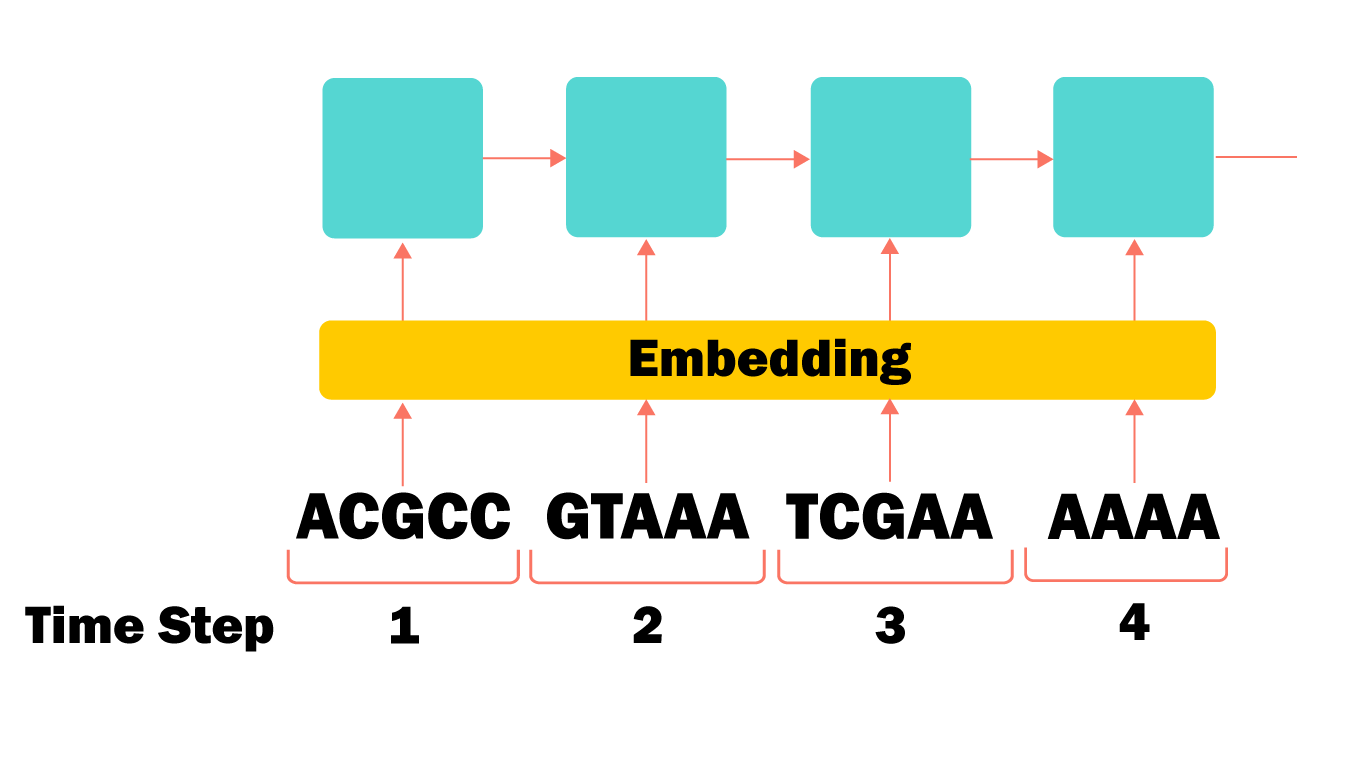
\includegraphics[width=\columnwidth]{imgs/encoder.PNG}
	\caption{Embedding Layer}
	\label{fig:encoder}
\end{figure}

\begin{figure}
	\centering
	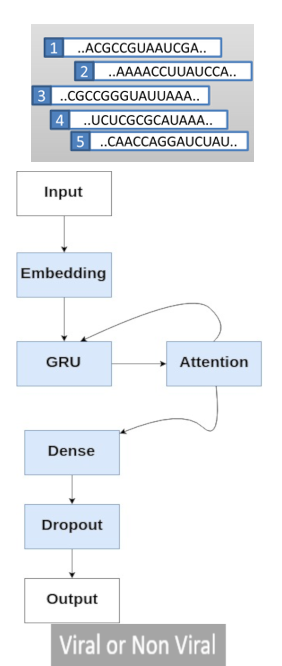
\includegraphics[width=0.75\columnwidth]{imgs/model_diagram.PNG}
	\caption{VirNet Model architecture}
	\label{fig:model_diagram}
\end{figure}

\section{Results}

\subsection{Results for generated fragments}
For the generated fragments of viruses and prokaryotes from RefSeq genomes. 
We tried different fragment length (n=100,500,1000,3000) with VirFinder and we found that VirFinder cannot identify viruses 100 bp. See figure \ref{fig:roc_auc_virfinder}.
We found our sequence model reached 85.12\% of accuracy whereas VirFinder tool obtained 75.61\% with the same training and testing data.

\begin{figure}
	\centering
	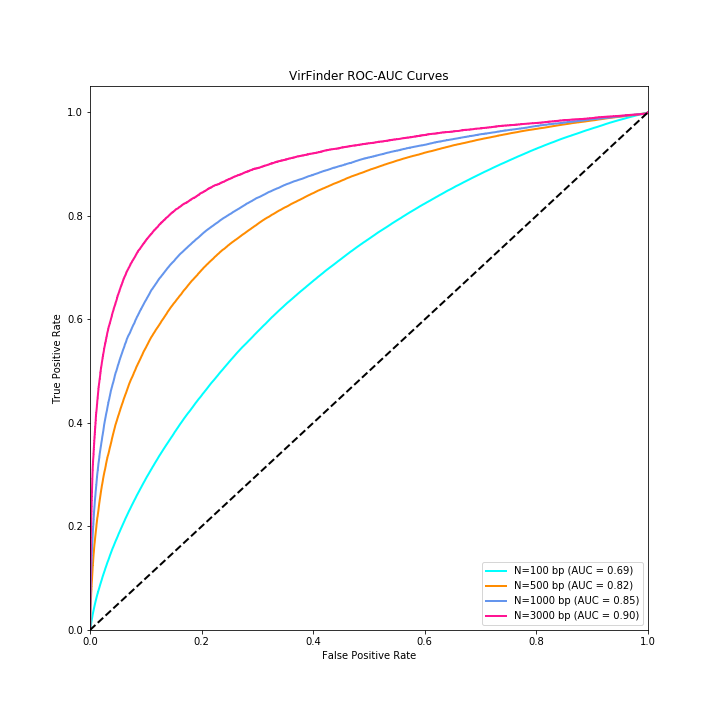
\includegraphics[width=\columnwidth]{imgs/roc_auc.png}
	\caption{VirFinder ROC-AUC curves}
	\label{fig:roc_auc_virfinder}
\end{figure}


\begin{table}[h!]
	\centering
	\begin{tabular}{||c c c c c||} 
		Length(N) &	Accuracy & Avg. Precision & Avg. Recall &	ROC-AUC \\ [0.5ex] 
		\hline\hline
		100 &	63.9\%	& 0.64 & 0.64 & 0.64 \\
		500 &	75.61\% &	0.76 & 0.76 & 0.75 \\
		1000 &	80.28\% & 0.82 & 0.80 & 0.78 \\
		3000 &	87.11\% & 0.88 & 0.87 & 0.83\\[1ex]
	\end{tabular}
	\caption{VirFinder Results on our test-set}
	\label{table:virfinder_results}
\end{table}


\subsection{Results for simulated metagenome}
We tried VirFinder on the simulated metagenomes and we found that VirFinder accuracy is arround 65\%. See figure \ref{fig:roc_auc_virfinder_simulated} and table \ref{table:virfinder_results_simulated}.

\begin{figure}
	\centering
	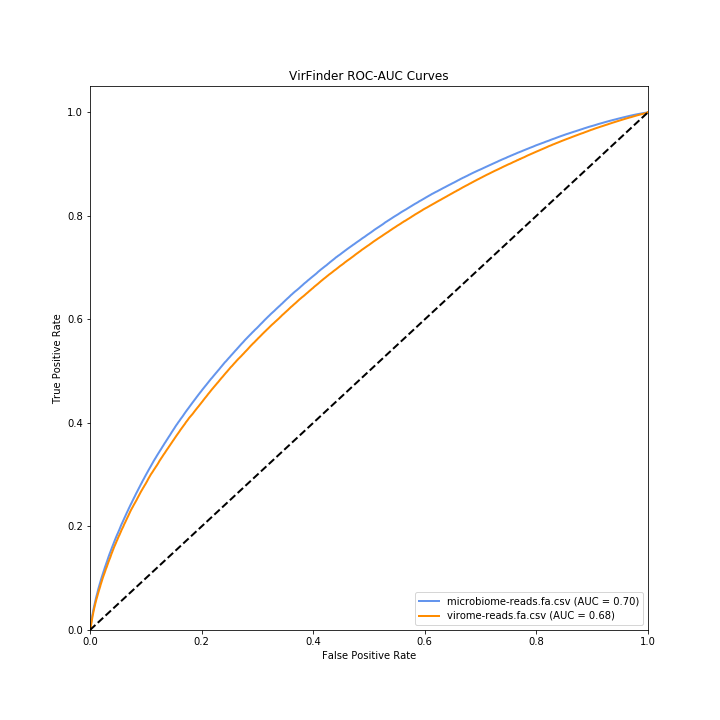
\includegraphics[width=\columnwidth]{imgs/roc_auc_simulated.png}
	\caption{VirFinder ROC-AUC curves on Simulated metagenomes}
	\label{fig:roc_auc_virfinder_simulated}
\end{figure}



\begin{table}[h!]
	\centering
	\begin{tabular}{||c c c c c||} 
		Length(N) &	Accuracy & Avg. Precision & Avg. Recall &	ROC-AUC \\ [0.5ex] 
		\hline\hline
		Virome &	62.77\%	& 0.72 & 0.63 & 0.63 \\
		Microbiome &	64.49\% &	0.72 & 0.64 & 0.64 \\ [1ex]
	\end{tabular}
	\caption{VirFinder Results on our Simulated Metagenomes}
	\label{table:virfinder_results_simulated}
\end{table}

\section{Discussion}

In our tool, there are no handmade features as the network will learn how to extract appropriate features for the raw data. It shows better accuracy as it is trained with the updated viral databases with a good statistical model. This helps us to generalize this model with all genomes and to make a generalized model for sequence classification. We also able to identify the short viral sequences as LSTM learns from the dependences between the input sequence. 
There is no evidence that these training prokaryotic genomes don't have viral infection or not. We need clean the training genomes to get better accuracy. Additionally, Using GPUs in this tool make it very fast and scalable with a large number of sequences. We found VirNet 16X faster than normal methods. 

\section{Conclusion}

We developed the first deep sequence network based on viral identification in large data. This tool will help us in expanding our knowledge in natural viral communities.

\section*{Acknowledgments}

We acknowledge Eng. Mayada Elsayed for designing the figures and Dr. Kiran Natra for her support.  


\section*{Availability of data}

VirNet is an open-source python package at https://github.com/alyosama/virnet. 
RefSeq genomes used are publicly available online via NCBI. All other generated data used in this study are available from the corresponding author on a request. 


\bibliography{scholar}
\bibliographystyle{plain}


\end{document}
